\chapter{Desarrollo y evaluación del modelo}
\label{cha:desarrollo}

En este capítulo, se abordará el desarrollo de los diferentes modelos de predicción de errores y el consecuente entrenamiento de los mismos. Para ello, se tomará como base el conjunto de datos resultante del Capítulo \ref{cha:analisis} y, específicamente, de la Sección \ref{sec:datasetfinal} (ver Tabla \ref{tab:datafinal}). Como paso previo al desarrollo, se introducirá una Sección de descripción de varias acciones de procesamiento adicional que son necesarias aplicar al conjunto de datos (ver Sección \ref{sec:adicional}).

\vspace{3mm}

Después, la organización del Capítulo se compone de otras dos partes diferenciadas en función de la naturaleza del aprendizaje que caracteriza a los modelos. Por un lado, se expondrán las técnicas de \gls{ml} empleadas para resolver la clasificación y predicción de errores (ver Sección \ref{sec:tecnicasml}). En el caso de este \gls{tfm}, se pone el foco en las técnicas \gls{rf} y \gls{svm}, cuyo funcionamiento fue descrito en las Secciones \ref{sec:mlrf} y \ref{sec:mlsvm}. Por otro lado, se realizará de la misma forma para las técnicas de \gls{dl} (ver Sección \ref{sec:tecnicasdl}). En particular, se detallará la configuración y la implementación de varias \gls{ann}s. Ambas Secciones comentadas se dividirán internamente, en base a la secuencia de pasos que se requieren para llevar a cabo el desarrollo completo de cada una de las técnicas.

\vspace{3mm}

Finalmente, se obtendrán una serie de resultados, que serán analizados y contrastados. En función de su precisión, se podrá determinar de forma concluyente qué modelo aporta una mayor efectividad en el diagnóstico y predicción de errores en una \gls{sg}.

%%%%%%%%%%%%%%%%%%%%%%%%%%%%%%%%%%%%%%%%%%%%%%%%%%%%%%%%%%%%%%
%%%%%%%%%%%%%%%%%%%%%%%%%%%%%%%%%%%%%%%%%%%%%%%%%%%%%%%%%%%%%%
\section{Preparación al desarrollo}
\label{sec:adicional}

En primera instancia, antes de proceder a desarrollar cualquier modelo, se debe concatenar en un mismo \textit{dataframe} el contenido de los 12 ficheros resultantes del Capítulo \ref{cha:analisis}. Esta agrupación, como se indicaba en la Sección \ref{sec:datasetfinal}, se abarca una cantidad total de 1931040 filas o intercambios etiquetados sobre los que entrenar los modelos. 

\vspace{3mm}

A partir de este conjunto de datos, como se pretende resolver un problema supervisado de clasificación, se deben seleccionar las características dependientes (\textit{X}), que suponen todas las columnas, exceptuando la referente a la etiqueta de error, `overflow', que es la característica independiente (\textit{y}). Después, se lleva a cabo un paso necesario de tratamiento de aquellas características que contienen datos categóricos. Particularmente, se observa que la columna `modelo' puede tomar dos valores en formato \textit{string}: `barabasi' o `waxman', en función del modelo de topología empleado. Ocurre de la misma forma para la fecha, la cual permite 12 posibles cadenas, al haberse probado 12 instantes temporales. Por ello, para poder manejar los datos proporcionados por ambas columnas, se requiere aplicar una transformación a valores numéricos mediante el método \textit{LabelEncoder}. Después, se añaden al \textit{dataframe} las nuevas columnas con los valores codificados y se desechan las originales.

\vspace{3mm}

\begin{lstlisting}[style=Python, caption={Codificación de los datos categóricos}]
  modelo = LabelEncoder().fit_transform(modelo) 
  datetime = LabelEncoder().fit_transform(datetime) 
\end{lstlisting}

\vspace{3mm}

Por consiguiente, se procede a analizar el resto de características del conjunto de datos (ver Tabla \ref{tab:datafinal}) y se toma la decisión de eliminar las columnas que hacen referencia a los diferentes valores de potencia (consumida, producida, carga neta), además de la marca de tiempo. Se aplica este paso por el motivo de que la condición de etiquetado de error en cada intercambio energético viene dada por el exceso de capacidad del enlace. Es decir, como se exponía en la Sección \ref{sec:etierror}, en la ejecución de las simulaciones en \gls{den2ne} se comprueba si cada valor de potencia que se intercambia entre dos nodos supera la capacidad del enlace que los une para activar la etiqueta. Como consecuencia, no sería correcto entrenar los modelos que se desarrollen en este Capítulo con los datos de potencia, puesto que se estaría reduciendo el análisis a los mismos y, por tanto, la clasificación y la predicción de errores. Esto produciría un \textit{overfitting} o sobreajuste de los modelos y los volvería ineficientes para cumplir los objetivos de este \gls{tfm}.

\vspace{3mm}

Tras los pasos anteriores de tratamiento y limpieza, ya se puede configurar el conjunto de datos y dividirlo en dos subconjuntos: uno se toma como entrada para entrenar el modelo (\textit{X\_train}, \textit{y\_train}) y otro, se trata como subconjunto de test para evaluar su funcionamiento (\textit{X\_test}, \textit{y\_test}). Se establece un tamaño de este último del 20\% del total del conjunto de datos.

\vspace{3mm}

\begin{lstlisting}[style=Python, caption={Codificación de los datos categóricos}]
  X_train, X_test, y_train, y_test = train_test_split(X, y, test_size = 0.2, random_state = 0)
\end{lstlisting}

\vspace{3mm}

Es importante en este punto estandarizar los datos para asegurar que todas las características poseen la misma escala. Para ello, se aplica el método \textit{StandardScaler} y se llevan a cabo dos acciones dedicadas al ajuste y a la transformación de los datos. Aunque la transformación del escalado se produce sobre los dos subconjuntos, el ajuste viene dado únicamente por los valores de promedio y de desviación estándar del subconjunto de entrenamiento. No se utiliza el de test para ello, puesto que se debe mantener ambos subconjuntos totalmente separados en este proceso. En otros términos, realizar el ajuste a partir de los datos del subconjunto de test podría llevar al \textit{overfitting} o sobreajuste de los modelos. Además, no se produciría una evaluación imparcial porque se estaría operando sobre "predicciones futuras".

\vspace{3mm}

\begin{lstlisting}[style=Python, caption={Estandarización de los subconjuntos}]
  sc = StandardScaler() 
  X_train = sc.fit_transform(X_train)
  X_test = sc.transform(X_test)
\end{lstlisting}

\vspace{3mm}

Una vez se estandarizan los subconjuntos de entrenamiento y de test, se concluye esta etapa de procesamiento adicional para poder comenzar a diseñar los modelos derivados de las técnicas de \gls{ml} y \gls{dl}.

%%%%%%%%%%%%%%%%%%%%%%%%%%%%%%%%%%%%%%%%%%%%%%%%%%%%%%%%%%%%%%
\section{Técnicas de \gls{ml}}
\label{sec:tecnicasml}

Teniendo en cuenta que los objetivos del presente \gls{tfm} se basan en la resolución de un problema de clasificación de errores, se toma la decisión de emplear \gls{rf} y \gls{svm}, como técnicas de aprendizaje supervisado. Para desarrollar diversos modelos en base a ambas, se requiere establecer la  secuencia de acciones a seguir: 

\begin{enumerate}
    \item Puntuación de características: Se diseña una primera versión o modelo por defecto de la técnica en cuestión para probar su funcionamiento. A partir del mismo, se aprecia las características que presentan mayor importancia en el proceso de clasificación, en base a la aplicación de varios métodos. 
    \item Optimización de hiperparámetros: Mediante la aplicación del método \textit{Grid Search}, se busca la mejor combinación de hiperparámetros de cada técnica para que el modelo resultante proporcione un rendimiento óptimo. 
    \item Selección de características: Una vez conocidos los hiperparámetros óptimos, se utilizan varias metodologías de reducción de la dimensionalidad para diseñar los nuevos modelos a partir de un volumen menor de datos.
    \item Ejecución del modelo y evaluación de resultados: Se extraen y se analizan los resultados de ejecución. Se validan en base a la precisión obtenida mediante la creación de la matriz de confusión y de la aplicación de la técnica \textit{K-Fold Cross Validation}.
\end{enumerate}

En esta Sección se implementarán dos nuevos \textit{notebooks}, \textit{rf.ipynb} y \textit{svm.ipynb}, los cuales tendrán como base el empleo de diferentes clases y métodos proporcionados por la biblioteca de software de código abierto \textit{scikit-learn} o \textit{sklearn}, además de otras librerías imprescindibles para el manejo de los datos, como son \textit{pandas}, \textit{matplotlib} o \textit{seaborn}. Se dispone de ambos ficheros en el repositorio\footnote{https://github.com/PaulaBartolomeMora/TFM/tree/main/den2ne} dedicado al desarrollo de este \gls{tfm}.

%%%%%%%%%%%%%%%%%%%%%%%%%%%%%%%%%%%%%%%%%%%%%%%%%%%%%%%%%%%%%%%%%%
\subsection{Random Forest (\acrshort{rf})}
\label{sec:rf}

\subsubsection{Puntuación de características}
\label{sec:rf1}

Se desarrolla una primera versión del clasificador basado en la técnica de \gls{rf}, \textit{RandomForestClassifier()} \cite{rfsklearn}, para visualizar las características que más repercuten en el proceso de clasificación de errores. En este modelo por defecto, se construyen un total de 10 estimadores o árboles y se determina el criterio de medición de la impureza a partir de la entropía (ver Sección \ref{sec:mlrf}). Después, se aplican dos métodos diferentes para puntuar la importancia que toman las características en el clasificador anterior. 

\vspace{3mm}

\begin{lstlisting}[style=Python, caption={Clasificador RF por defecto}]
  classifier = RandomForestClassifier(n_estimators = 10, criterion = 'entropy', random_state = 0) 
  classifier.fit(X_train, y_train)
\end{lstlisting}
  
\vspace{3mm}

Por un lado, se estima la importancia de las características del conjunto, a partir del atributo \textit{feature\_importances\_}, proporcionado por el clasificador. En este caso, el cálculo se realiza a partir de la media y de la desviación estándar de la disminución de la impureza que se produce dentro de cada árbol. Como se representa en la Figura \ref{fig:imp1}, se devuelve un array con los valores de importancia relativa asignados a las características y cuyo sumatorio es igual a 1. En este caso, se visualiza una gran incidencia de la distancia, seguida de los parámetros resultantes de \gls{den2ne}, \textit{total\_balance} y \textit{abs\_flux}, que hacen referencia a la carga que presenta el nodo \textit{gateway} tras el balance y al flujo total de recursos intercambiados en el proceso de distribución energética.

\vspace{3mm}

Sin embargo, con este método surgen cierto sesgo hacia las características que presentan alta cardinalidad, o en otros términos, una gran cantidad de valores únicos. Esto se debe a que generan nodos de división con mayor profundidad en los árboles, puesto que existen más opciones de separación del conjunto de datos. Por lo tanto, este tipo de características pueden recibir una puntuación más inflada. Teniendo esto en cuenta, se decide cuantificar la importancia también por el método de permutación (\textit{permutation\_importance}). Como se puede ver en la Figura \ref{fig:imp2}, en este caso, los parámetros resultantes de \gls{den2ne}, \textit{total\_balance} y \textit{abs\_flux}, siguen presentando puntuaciones altas, pero ahora también, las longitudes de las etiquetas de los nodos y la capacidad del enlace. \cite{importance}

\begin{figure}[H]
  \centering
  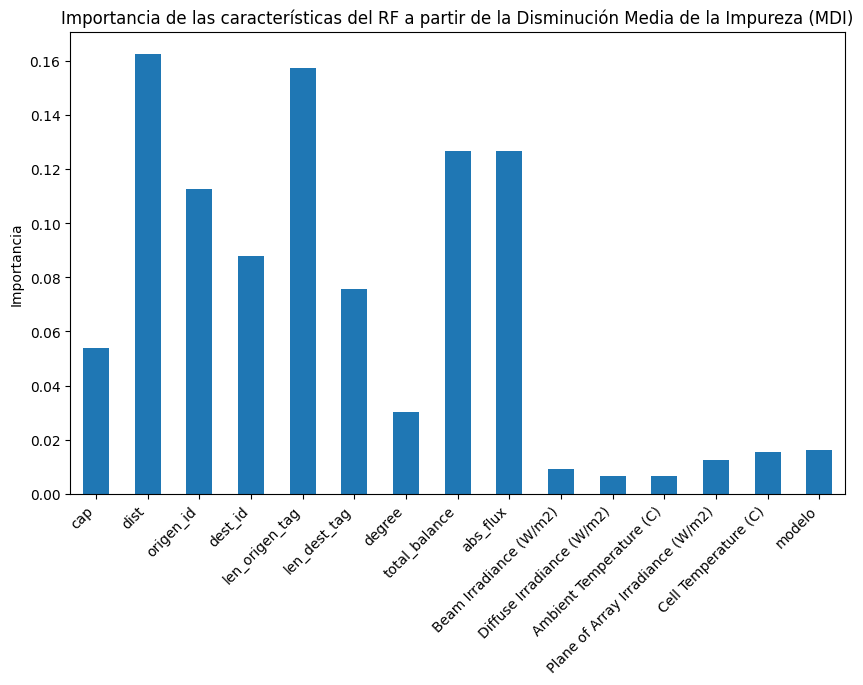
\includegraphics[width=1\textwidth]{img/desarrollo/rf/importance1.png}
  \caption{Puntuación de características del \acrshort{rf} mediante el atributo \textit{feature\_importances\_}}
  \label{fig:imp1}
\end{figure}

\begin{figure}[H]
  \centering
  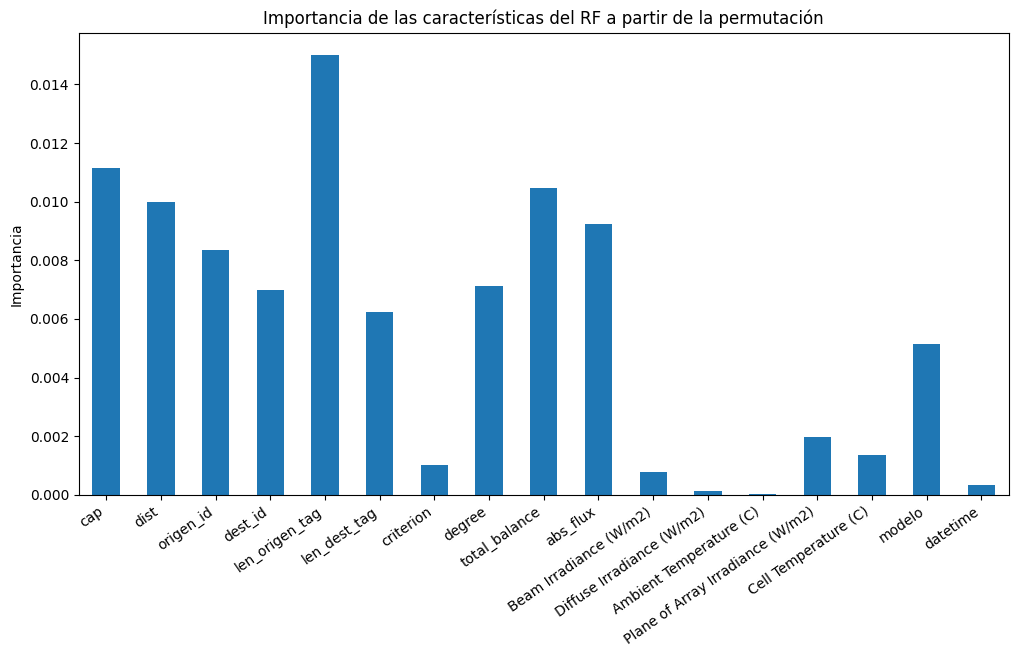
\includegraphics[width=1\textwidth]{img/desarrollo/rf/importance2.png}
  \caption{Puntuación de características del \acrshort{rf} mediante el método \textit{permutation\_importance}}
  \label{fig:imp2}
\end{figure}

En este segundo método los valores de las características se permutan una a una aleatoriamente y se evalúa en cada iteración los resultados del clasificador. Por tanto, cuando la variación de valores de una característica decrementa de forma considerable la precisión del modelo, puntúa una mayor importancia. Esta técnica es útil porque proporciona una evaluación imparcial de la importancia de las características. 

\subsubsection{Optimización de hiperparámetros}
\label{rf2}

Los hiperparámetros de un modelo se tratan de los parámetros de configuración o argumentos que son incluidos en el constructor de la clase del estimador o clasificador. En el caso del \gls{rf}, como ya se había introducido en el diseño del modelo por defecto, se pone el foco en dos hiperparámetros principales: el número de estimadores o árboles y el criterio de medición de la impureza. Para encontrar los valores que construyen el modelo óptimo de \gls{rf}, es preciso emplear la técnica \textit{Grid Search} \cite{gridsearch} y, específicamente, la clase \textit{GridSearchCV()} \cite{gridsearch2}. Esta realiza una búsqueda exhaustiva a partir de la definición de una cuadrícula de hiperparámetros para el estimador y extrae la combinación de valores que aporta una mayor precisión. Por ello, es necesario primero, definir en un diccionario una serie de valores para los dos hiperparámetros que se pretenden optimizar en el nuevo clasificador.

\vspace{3mm}

\begin{lstlisting}[style=Python, caption={Cuadrícula de parámetros RF}]
  param_grid = {
    'n_estimators': [10, 25, 50, 75, 100],
    'criterion': ['entropy', 'gini']
  }
\end{lstlisting}

\vspace{3mm}

Por consiguiente, se crea el objeto de la clase \textit{GridSearchCV()} y se determina el esquema de validación cruzada (\textit{cross validation}) de este mediante el parámetro \textit{cv}. En este caso, toma un valor de 5 y define el número de pliegues (\textit{folds}) que se van a utilizar para dividir el conjunto de datos y evaluar las combinaciones de los hiperparámetros. De la misma forma, se especifican el resto de parámetros, como la métrica para evaluar el rendimiento del modelo en cada iteración, que viene dada por la precisión global obtenida (\textit{accuracy}). 

\vspace{3mm}

Una vez creado el objeto, se ajusta al conjunto de datos de entrenamiento. Este proceso, a partir de los atributos \textit{best\_score\_} y \textit{best\_params\_}, aporta a la salida cuál es la mejor combinación de parámetros de todas las probadas y qué valor de precisión alcanza la misma. En este caso, se obtiene una precisión del 99,18\% con un clasificador basado en 100 estimadores y en el criterio de entropía. 

\vspace{3mm}

\begin{lstlisting}[style=Python, caption={Construcción del objeto \textit{GridSearchCV()}}]
  grid_search = GridSearchCV(estimator = classifier,
                            param_grid = param_grid,
                            scoring = 'accuracy',
                            cv = 5,
                            n_jobs = -1)

  grid_search.fit(X_train, y_train)
\end{lstlisting}

\vspace{3mm}

Sin embargo, para llevar a cabo un análisis en mayor profundidad de los resultados, se hace uso del atributo \textit{cv\_results\_}, que proporciona un diccionario con toda la información útil de la búsqueda. Principalmente, este análisis se centra en los valores de precisión obtenidos de todos los modelos y en los tiempos promedios que han sido necesarios para ajustar los mismos al conjunto de entrenamiento. Como se puede apreciar en la Tabla \ref{tab:rfgs}, se presentan variaciones muy pequeñas en los valores de precisión obtenida (\textit{mean\_test\_score}) para las diferentes combinaciones de parámetros.

\vspace{3mm}

\begin{table}[H]
  \centering
  \begin{subtable}{0.45\linewidth}
    \centering
    \begin{tabular}{|>{\columncolor[HTML]{EFEFEF}}c |c|c|}
      \hline
      \textit{\begin{tabular}[c]{@{}c@{}}Criterio /\\ Nº estimadores\end{tabular}} & \cellcolor[HTML]{EFEFEF}\textit{Entropía} & \cellcolor[HTML]{EFEFEF}\textit{Gini} \\ \hline
      10 & 99,07 & 99,02 \\ \hline
      25 & 99,16 & 99,14 \\ \hline
      50 & 99,16 & 99,15 \\ \hline
      75 & 99,17 & 99,17 \\ \hline
      100 & 99,18 & 99,16 \\ \hline
    \end{tabular}
    \caption{Precisión (\%) (\textit{mean\_test\_score})}
    \label{tab:rfgs}
  \end{subtable}
  \hfill
  \begin{subtable}{0.45\linewidth}
    \centering
    \begin{tabular}{|>{\columncolor[HTML]{EFEFEF}}c |c|c|}
      \hline
      \textit{\begin{tabular}[c]{@{}c@{}}Criterio /\\ Nº Estimadores\end{tabular}} & \cellcolor[HTML]{EFEFEF}\textit{Entropía} & \cellcolor[HTML]{EFEFEF}\textit{Gini} \\ \hline
      10 & 147 & 146 \\ \hline
      25 & 373 & 382 \\ \hline
      50 & 747 & 761 \\ \hline
      75 & 1072 & 1002 \\ \hline
      100 & 1439 & 987 \\ \hline
    \end{tabular}
    \caption{Tiempo (s) (\textit{mean\_fit\_time})}
    \label{tab:rfgs2}
  \end{subtable}
  \caption{Resultados extraídos del atributo \textit{cv\_results\_} del \textit{Grid Search} en el \acrshort{rf}}
  \label{tab:rfgs_combined}
\end{table}

\vspace{3mm}

No obstante, en el caso de los tiempos (\textit{mean\_fit\_time}), como es coherente, sí que se observan grandes diferencias. En la Tabla \ref{tab:rfgs2} se visualiza cómo se incrementa la duración de la búsqueda proporcionalmente al número de estimadores que se emplea. Esta métrica es importante también tenerla en cuenta para determinar el modelo óptimo, ya que a partir de la aplicación de 25 estimadores, la precisión no mejora de forma considerable. Por lo tanto, tras analizar los resultados, se puede expresar de forma concluyente que la mejor opción de modelo a emplear viene dada por un \gls{rf} basado en 25 estimadores o árboles y en el criterio de medición de la impureza a partir de la entropía.

\subsubsection{Selección de características}
\label{sec:rf3}

El proceso de selección de características viene dado por la necesidad de reducir las dimensiones del conjunto de datos y eliminar la información irrelevante o redundante que introduce ruido en el conjunto. En esta Sección, se expone el empleo de tres técnicas diferentes con el fin de realizar posteriormente un análisis comparativo de los resultados que se obtienen tras aplicar cada una de ellas al conjunto de datos (ver Sección \ref{sec:rf4}).

\vspace{3mm}

En primer lugar, se introduce la técnica de eliminación recursiva de características con validación cruzada (del inglés \gls{rfecv}) \cite{rfecv}. Esta se basa en la ejecución de un proceso iterativo para ir desechando las características que tienen menor influencia en los resultados de precisión, hasta que el rendimiento del modelo deja de mejorar significativamente. 

\vspace{3mm}

Por este motivo, además de proveer a su salida la lista de características más importantes, es capaz de indicar cuál es el número óptimo de características que se debería aplicar para maximizar la precisión en el entrenamiento del modelo, a la vez que se minimiza el volumen de datos en el mismo. En este caso, el \gls{rfecv} se configura con un total de 5 divisiones (\textit{cv}) del conjunto de datos para llevar a cabo el proceso de evaluación. Además, se determina la eliminación de una de las características disponibles en cada iteración (\textit{step}). 

\vspace{3mm}

\begin{lstlisting}[style=Python, caption={Aplicación del \acrshort{rfecv}}]
  rfecv = RFECV(estimator=classifier, step=1, cv=5, scoring='accuracy') 
  rfecv = rfecv.fit(X_train, y_train)
\end{lstlisting}

\vspace{3mm}

\begin{lstlisting}[language=bash, style=Python, caption={Resultados del \acrshort{rfecv}}]
  Nº óptimo de features : 8
  Selected features : Index(['cap', 'dist', 'origen_id', 'dest_id', 'len_origen_tag', 'len_dest_tag', 'total_balance', 'abs_flux'], dtype='object')
\end{lstlisting}

\vspace{3mm}

Se puede visualizar el proceso de evaluación del número de características gráficamente en la Figura \ref{fig:rfecv}, en la cual se representa cómo la precisión del modelo es máxima cuando se utilizan 8. Por otro lado, en cuanto a la lista de características proporcionada por el \gls{rfecv}, es preciso llevar a cabo una comparación con las puntuaciones obtenidas en la Sección \ref{sec:rf1}. Volviendo a las Figuras \ref{fig:imp1} y \ref{fig:imp2}, se confirma que, exceptuando ligeras variaciones, la lista de características es coherente con las que presentan mayor grado de importancia.

\vspace{3mm}

\begin{figure}[H]
  \centering
  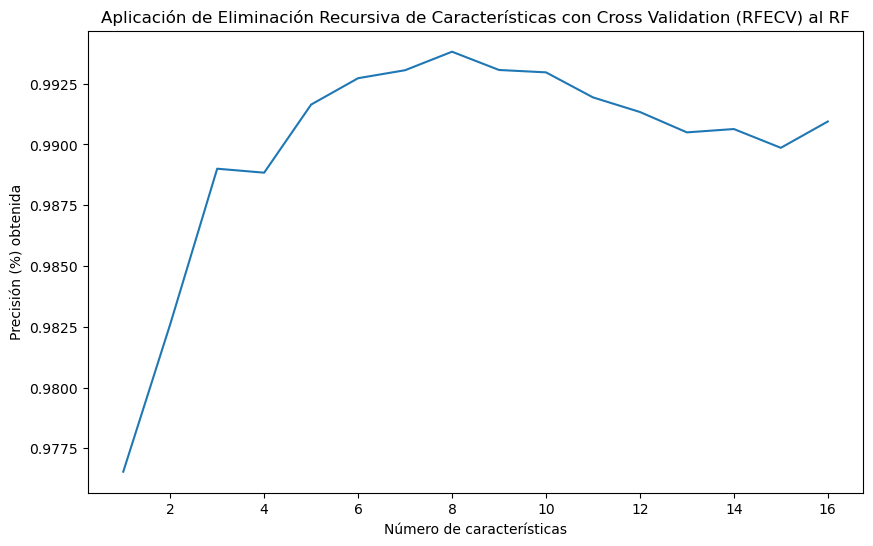
\includegraphics[width=0.85\textwidth]{img/desarrollo/rf/rfecv.png}
  \caption{Análisis de la precisión del modelo en función del número de características empleadas}
  \label{fig:rfecv}
\end{figure}

Por consiguiente, se entra en el funcionamiento de la segunda técnica a emplear, denominada como Selección Invariante de Características (del inglés \textit{Univariate feature selection}) o, también denominado, \textit{kBest} \cite{kbest}. En este caso, la operativa incluye un escalado previo de las características, para que sus valores se sitúen en un rango [0, 1]. Después, se declara el objeto de la clase especificada para la técnica en cuestión, \textit{SelectKBest()}, y se determina cuántas características se pretenden seleccionar del total que provee el conjunto. A diferencia del \gls{rfecv}, para conocer cuál es el número óptimo en la selección invariante de características, es preciso basarse en la prueba y error, puesto que no se proporciona este dato a la salida. Por ello, a modo comparativo, se produce el entrenamiento del conjunto de datos en base a k=5 y a k=8 características. 

\vspace{3mm}

\begin{lstlisting}[style=Python, caption={Aplicación del \textit{kBest}}]
  scaler = MinMaxScaler() # Escalado de las características en el rango [0, 1]
  kbest = SelectKBest(chi2, k=8)
  kbest = kbest.fit(scaler.fit_transform(X_train), y_train)
\end{lstlisting}

\vspace{3mm}

Una vez que se extraen, a partir del atributo \textit{feature\_names\_in}, aquellas características con mayor puntuación, se procede a transformar los conjuntos de entrenamiento y de test. Si se compara la lista proporcionada por el atributo anterior con las puntuaciones de las Figuras \ref{fig:imp1} y \ref{fig:imp2}, se puede comprobar que esta técnica no estan precisa como en el caso del \gls{rfecv}, puesto que se seleccionan algunas características que no presentan tan buenas puntuaciones. Por ello, se estima a priori, que la implementación de la selección invariante no mejorará los resultados de precisión que se esperan con \gls{rfecv}.

\vspace{3mm}

\begin{lstlisting}[language=bash, style=Python, caption={Resultados del \textit{kBest} para \textit{k=8}}]
  Selected features : Index(['cap', 'len_origen_tag', 'len_dest_tag', 'degree', 'abs_flux', 'Beam Irradiance (W/m2)', 'Plane of Array Irradiance (W/m2)', 'Cell Temperature (C)'], dtype='object')       
\end{lstlisting}

\vspace{3mm}

Por último, se introduce una técnica, que no es estrictamente de selección de características, pero que se incluye en esta Sección, puesto que el objetivo que se persigue viene dado por la reducción de la dimensionalidad del conjunto de datos. Se denomina como Análisis de Componentes Principales (del inglés \gls{pca}) \cite{pca} y se basa en la aplicación de la técnica matemática de Descomposición en Valores Singulares (del inglés \gls{svd}). Es decir, su funcionamiento consiste en la búsqueda de las direcciones principales de variación (k vectores) del conjunto de datos para construir una matriz de proyección, que establezca un nuevo espacio de características de k dimensiones.

\vspace{3mm}

No obstante, antes de aplicar el ajuste y la transformación al conjunto de datos a partir del \gls{pca}, se debe configurar el número de componentes a emplear. Para ello, se utiliza el "método del codo" (del inglés \textit{Elbow Method}) para identificar el punto o "codo" en el que el aumento del número de componentes no aporta mejoras significativas en el valor de la varianza. 

\vspace{3mm}

\begin{figure}[H]
  \centering
  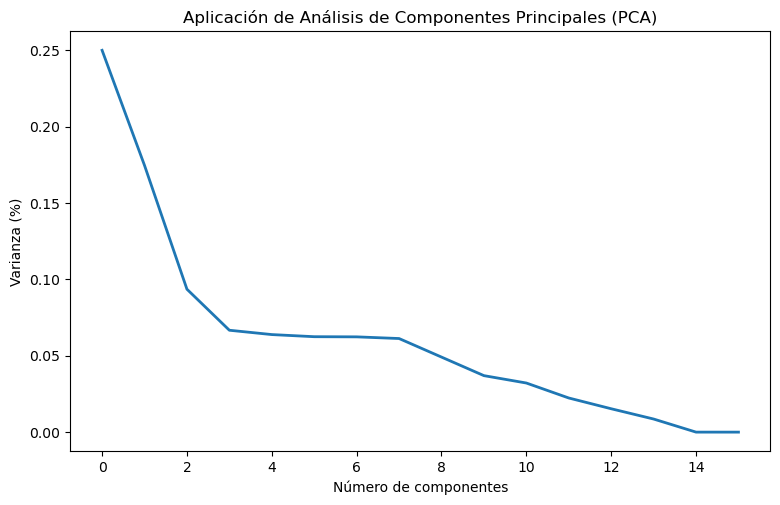
\includegraphics[width=0.85\textwidth]{img/desarrollo/pca.png}
  \caption{Análisis de la varianza en función del número de componentes empleadas en el \gls{pca}}
  \label{fig:pca}
\end{figure}

\vspace{3mm}

Como se representa en la Figura \ref{fig:pca}, en n=4 componentes, se produce el estancamiento más considerable de la varianza, en un valor del 6\% aproximadamente. Se puede visualizar que, para el caso de n=2 componentes, también ocurre pero en menor medida. Por ello, para comparar los resultados posteriormente, se considera aplicar el \gls{pca} en función de ambos números.

\subsubsection{Ejecución del modelo y evaluación de resultados}
\label{sec:rf4}

Por un lado, como se ha detallado en la Sección \ref{rf2}, el modelo que se considera más adecuado y, por tanto, sobre el que se decide trabajar, viene dado por la configuración de 25 estimadores y el criterio de la entropía.

\vspace{3mm}

\begin{lstlisting}[style=Python, caption={Clasificador RF seleccionado}]
  classifier = RandomForestClassifier(n_estimators = 25, criterion = 'entropy', random_state = 0) 
  classifier.fit(X_train, y_train)
\end{lstlisting}
  
\vspace{3mm}

Por otro lado, en la Sección \ref{sec:rf3} se han expuesto varias propuestas de selección de características o de reducción de dimensiones del conjunto de datos. Esta Sección viene dada por la necesidad de aplicar un proceso de evaluación sobre las diferentes implementaciones del modelo de \gls{rf} seleccionado con el fin de analizar el rendimiento y precisión que proporcionan cada una de ellas. 

\vspace{3mm}

No obstante, en primera instancia, se procede a ejecutar el modelo de \gls{rf}, tanto empleando las diferentes opciones de reducción de dimensiones del conjunto de datos, como sin aplicar ninguna de ellas para realizar la comparativa. A modo de proveer una mayor comprensión del entrenamiento que se produce, se incluye la lógica de representación de los estimadores o árboles de decisión del \gls{rf}, mediante el empleo del método de conversión \textit{export\_graphviz} \cite{graphviz2} y la herramienta de generación de grafos, \textit{WebGraphViz}. En la Figura \ref{fig:tree} se expone uno de los árboles que se construyen en este proceso.

\vspace{3mm}

Por consiguiente, una vez ejecutado, se puede llevar a cabo el proceso de evaluación, que consta del empleo de dos métodos: la matriz de confusión y el \textit{K-Fold Cross Validation}. La matriz de confusión \cite{cm} es un método de gran utilidad cuando se trabaja con técnicas de clasificación binaria, como se produce en este caso para detectar y predecir los intercambios energéticos con errores. Permite analizar la precisión del modelo mediante la organización de las predicciones en cuatro categorías diferentes (ver Figura \ref{fig:confusion}): 

\begin{itemize}
  \item Verdaderos positivos (TP): Predicciones correctas de intercambios sin errores.
  \item Falsos positivos (FP): Predicciones incorrectas de intercambios sin errores.
  \item Verdaderos negativos (TN): Predicciones correctas de intercambios con errores.
  \item Falsos negativos (FN): Predicciones incorrectas de intercambios con errores.
\end{itemize}

\begin{sidewaysfigure}
  \centering
  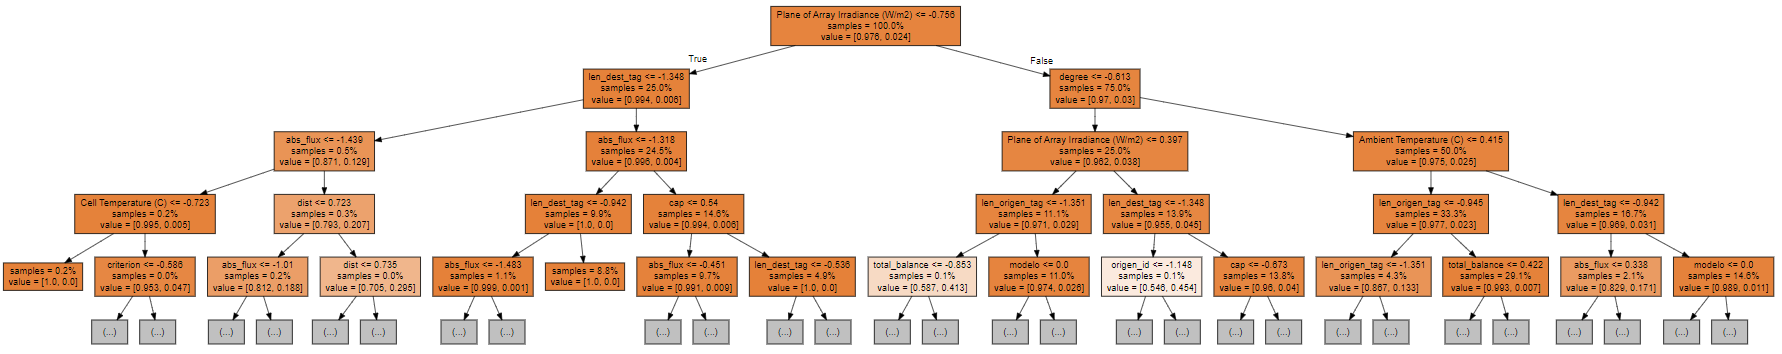
\includegraphics[width=1\textwidth]{img/desarrollo/rf/tree2.png}
  \caption{Ejemplo gráfico de un estimador o árbol del \gls{rf} \cite{graphviz}}
  \label{fig:tree}
\end{sidewaysfigure}

\begin{figure}[H]
  \centering
  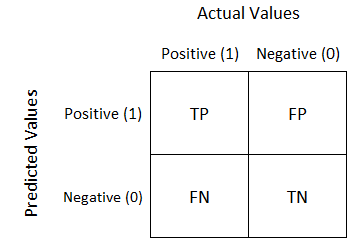
\includegraphics[width=0.45\textwidth]{img/desarrollo/rf/confusion.png}
  \caption{Matriz de confusión \cite{cm2}}
  \label{fig:confusion}
\end{figure}

\vspace{3mm}

A través de las categorías definidas en la matriz, se pueden obtener cuatro métricas de evaluación: 

\vspace{3mm}

\begin{itemize}
  \item \textit{Accuracy}: Mide la proporción de predicciones correctas en relación con el total y evalúa el rendimiento general de un modelo de clasificación.
  \[\textit{Accuracy} = \frac{{TP + TN}}{{TP + TN + FP + FN}}\]
  \item \textit{Precision}: Mide la proporción de verdaderos positivos entre todas las instancias clasificadas como positivas.
  \[\text{Precision} = \frac{{TP}}{{TP + FP}}\]
  \item \textit{Recall}: Mide la proporción de verdaderos positivos identificados correctamente entre todas las instancias que son realmente positivas. 
  \[\text{Recall} = \frac{{TP}}{{TP + FN}}\]
  \item \textit{F1 Score}: Combina las dos métricas anteriores, tomando en cuenta tanto los falsos positivos como los falsos negativos.
  \[\text{F1 Score} = \frac{{2 \times \text{Precision} \times \text{Recall}}}{{\text{Precision} + \text{Recall}}}\]
\end{itemize}

\begin{lstlisting}[style=Python, caption={Implementación de la matriz de confusión}]
  cm = confusion_matrix(y_test, y_pred)
  accuracy_score(y_test, y_pred)
\end{lstlisting}

\vspace{3mm}

Por tanto, con la aplicación de la matriz de confusión, se extraen los resultados expuestos en la Tabla \ref{tab:rfcm}. En la misma se puede visualizar la cantidad de predicciones, en función de cada una de las categorías de la matriz y los valores obtenidos del cálculo de las métricas anteriores. A priori, si solo se pone el foco en la precisión global del modelo (\textit{Accuracy}), las opciones que proveen valores más altos son la que no aplica ningún método de reducción de dimensiones y que por tanto, opera con todas las características del conjunto, y la que emplea la técnica \gls{rfecv}. 

\vspace{3mm}

En el caso de la precisión de los valores positivos (\textit{Precision}) o, en otros términos, de las instancias que se predicen como erróneas, vuelve a ocurrir de la misma manera. A pesar de que para la métrica \textit{Accuracy} los valores de todas las opciones son relativamente parecidos, para \textit{Precision} se visualizan grandes diferencias. Por ejemplo, el empleo de un \gls{pca} con n=2 provee un buen valor de precisión global (97,55\%), pero no tiene un buen rendimiento en la clasificación de los errores (12,52\%). En consecuencia, el valor del \textit{Recall} también es muy pequeño en este caso (0,67\%). El resto de opciones, exceptuando las dos primeras, ya mencionadas anteriormente, presentan también porcentajes bajos, suponiendo un coste alto de predicción de errores. 

\vspace{3mm}

\begin{table}[H]
  \centering
  \begin{tabular}{|c|c|c|c|c|c|c|c|c|}
  \hline
  \rowcolor[HTML]{EFEFEF} 
  \textit{\begin{tabular}[c]{@{}c@{}}Matriz\\ de confusión\end{tabular}} & \cellcolor[HTML]{EFEFEF}\textit{TN} & \textit{FP} & \textit{FN} & \textit{TP} & \textit{Accuracy} & \textit{Precision} & \textit{Recall} & \textit{F1 Score} \\ \hline
  \cellcolor[HTML]{EFEFEF}\textit{Sin aplicar} & 376745 & 399 & 2332 & 6732 & 99,29 & 94,40 & 74,27 & 83,16 \\ \hline
  \cellcolor[HTML]{EFEFEF}\textit{RFECV} & 376699 & 445 & 1717 & 7347 & 99,44 & 04,28 & 81,05 & 87,17 \\ \hline
  \cellcolor[HTML]{EFEFEF}\textit{kbest (n=5)} & 376555 & 589 & 7927 & 1137 & 97,79 & 65,97 & 12,55 & 21,08 \\ \hline
  \cellcolor[HTML]{EFEFEF}\textit{kbest (n=8)} & 375027 & 2117 & 6583 & 2481 & 97,74 & 53,95 & 27,37 & 36,32 \\ \hline
  \cellcolor[HTML]{EFEFEF}\textit{PCA (n=2)} & 376718 & 426 & 9003 & 61 & 97,55 & 12,52 & 00,67 & 01,27 \\ \hline
  \cellcolor[HTML]{EFEFEF}\textit{PCA (n=4)} & 376684 & 460 & 7015 & 2049 & 98,06 & 81,66 & 22,60 & 35,41 \\ \hline
  \end{tabular}
  \caption{Resultados de aplicación de la matriz de confusión al \gls{rf}}
  \label{tab:rfcm}
\end{table}

\vspace{3mm}

De la misma forma, se puede visualizar que para la métrica \textit{F1 Score} se esperan resultados relativamente cercanos al \textit{Recall}. Al considerarse tanto los falsos positivos, como los falsos negativos, produce que la obtención de un porcentaje significativamente pequeño indique una baja \textit{Precision} y \textit{Recall} conjuntamente. 

\vspace{3mm}

Por otro lado, en cuanto al método \textit{K-Fold Cross Validation} \cite{kfold}, se emplea la misma operativa que en el \textit{Grid SearchCV}. Como su nombre indica, se basa en un esquema de validación cruzada (\textit{cross validation}) y se divide el conjunto de datos en un total de 5 pliegues para evaluar el rendimiento del modelo. En la Tabla \ref{tab:rfk}, se determinan los resultados de su aplicación y, como se puede visualizar, los valores de precisión global son prácticamente iguales a los obtenidos anteriormente en la matriz de confusión. Por tanto, mediante el empleo de las dos técnicas y el análisis expuesto, se confirma que las opciones con mejores resultados hacen referencia a la que no se aplica ningún método de reducción de dimensiones y a la que emplea \gls{rfecv}, siendo esta última la que proporciona un rendimiento óptimo.

\vspace{3mm}

\begin{lstlisting}[style=Python, caption={Implementación del \textit{K-Fold Cross Validation}}]
accuracies = cross_val_score(estimator = classifier, X = X_train, y = y_train, cv = 5)
\end{lstlisting}

\vspace{3mm}

\begin{table}[H]
  \centering
  \begin{tabular}{|c|c|c|c|c|c|c|c|c|}
  \hline
  \rowcolor[HTML]{EFEFEF} 
  \textit{\begin{tabular}[c]{@{}c@{}}K-Fold\\ Cross Validation\end{tabular}} & \cellcolor[HTML]{EFEFEF}\textit{Accuracy (\%)} & \textit{Standard Deviation (\%)} \\ \hline
  \cellcolor[HTML]{EFEFEF}\textit{Sin aplicar} & 99,30 & 0,02 \\ \hline
  \cellcolor[HTML]{EFEFEF}\textit{RFECV} & 99,47 & 0,02 \\ \hline
  \cellcolor[HTML]{EFEFEF}\textit{kbest (n=5)} & 97,80 & 0,02 \\ \hline
  \cellcolor[HTML]{EFEFEF}\textit{kbest (n=8)} & 97,79 & 0,01 \\ \hline
  \cellcolor[HTML]{EFEFEF}\textit{PCA (n=2)} & 97,35 & 0,01 \\ \hline
  \cellcolor[HTML]{EFEFEF}\textit{PCA (n=4)} & 98,04 & 0,00 \\ \hline
  \end{tabular}
  \caption{Resultados de aplicación del \textit{K-Fold Cross Validation} al \gls{rf}}
  \label{tab:rfk}
\end{table}





%%%%%%%%%%%%%%%%%%%%%%%%%%%%%%%%%%%%%%%%%%%%%%%%%%%%%%%%%%%%%%%%%%
\subsection{Support Vector Machines (\acrshort{svm})}
\label{sec:svm}

\subsubsection{Puntuación de características}
\label{sec:svm1}

Para la técnica de \gls{svm}, también se procede a desarrollar una primera versión de clasificador para poder visualizar la importancia que toman las características en el mismo. En este caso, se trata de la clase \textit{SVC()} \cite{svc} y se inicializa un objeto de la misma con la definición por defecto de un kernel radial o gaussiano (\gls{rbf}), ya que se trabaja con un conjunto de datos no linearmente separables y que resulta complejo de operar si no se aumenta la dimensionalidad del espacio (ver Sección \ref{sec:mlsvm}). 

\vspace{3mm}

Adicionalmente, \textit{SVC()} determina valores por defecto de los hiperparámetros \textit{C} y \textit{gamma}, que hacen referencia respectivamente, a la regularización del modelo y al impacto que produce cada instancia de entrenamiento en el proceso de clasificación. El clasificador se ejecuta, se entrena con el conjunto de datos y, por consiguiente, se le aplican dos métodos de puntuación de características. Cabe destacar que, en esta primera versión del clasificador del \gls{svm}, el proceso de entrenamiento se caracteriza por presentar una duración mucho mayor que con el \gls{rf} --------------.

\vspace{3mm}

\begin{lstlisting}[style=Python, caption={Clasificador SVM por defecto}]
  classifier = SVC(kernel = 'rbf', random_state = 0) #por defecto C=1, gamma='scale' o 'auto'
  classifier.fit(X_train, y_train)
\end{lstlisting}
  
\vspace{3mm}

Por un lado, se estima la importancia de las características a partir de la distancia que tienen hacia los vectores de soporte. En este caso es preciso basarse en los atributos \textit{support\_vectors\_} y \textit{dual\_coef\_}, que proporcionan la información sobre los vectores soporte que se han definido en el \gls{svm} y los multiplicadores de \textit{Lagrange} asociados. El resultado se expone en la Figura \ref{fig:imp3}, en la cual se visualiza cómo las longitudes de las etiquetas origen y destino inciden en la clasificación significativamente, ya que el resto de características tienen puntuaciones mucho más bajas.

\vspace{3mm}

Por otro lado, al igual que se ha expuesto para el \gls{rf} (ver Sección \ref{sec:rf1}), se incluye el análisis a partir del método de la permutación (\textit{permutation\_importance}). En este caso, las longitudes de las etiquetas siguen siendo predominantes, pero las características que hacen referencia a la capacidad y al flujo total de energía resultante de \gls{den2ne} (\textit{abs\_flux}) también presentan valores de puntuaciones a considerar.

\begin{figure}[H]
    \centering
    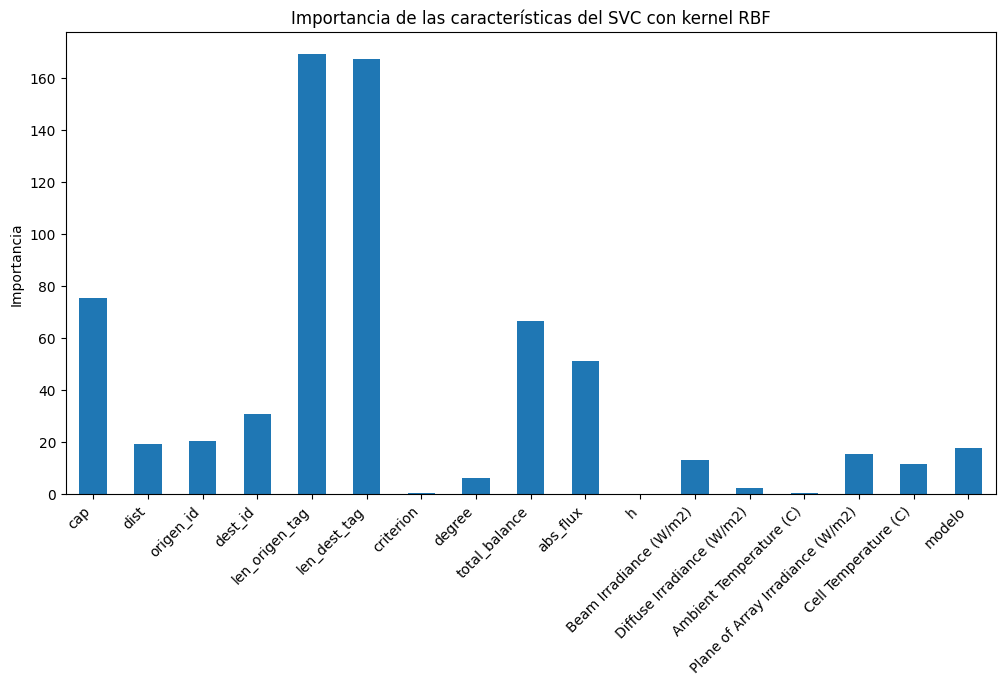
\includegraphics[width=1\textwidth]{img/desarrollo/svm/importance3.png}
    \caption{Puntuación de características del \acrshort{svm} mediante los atributos \textit{support\_vectors\_} y \textit{dual\_coef\_}}
    \label{fig:imp3}
\end{figure}
  
\begin{figure}[H]
    \centering
    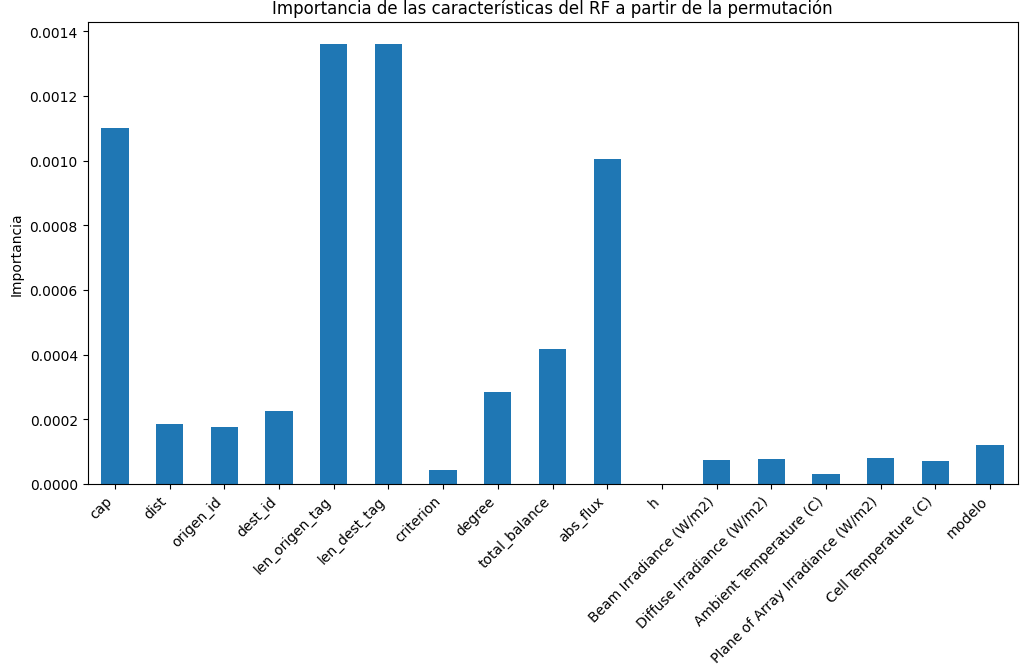
\includegraphics[width=1\textwidth]{img/desarrollo/svm/importance4.png}
    \caption{Puntuación de características del \acrshort{svm} mediante el método \textit{permutation\_importance}}
    \label{fig:imp4}
\end{figure}

\subsubsection{Optimización de hiperparámetros}

Para modelar un \gls{svm} óptimo se centra el estudio en dos hiperparámetros: el tipo de kernel a aplicar y el parámetro de regularización \textit{C}. En el caso de \textit{gamma}, mencionada anteriormente, es indiferente su configuración, puesto que los datos del conjunto han sido previamente escalados (ver Sección \ref{sec:adicional}) y las dos opciones posibles de \textit{gamma} ('scale' o 'auto') solo se diferencian en si se aplica o no la varianza de los datos en el cálculo del parámetro. Por lo tanto, desechando el análisis de \textit{gamma}, se aplica el método \textit{Grid Search} para realizar la búsqueda de la combinación óptima de hiperparámetros.

\vspace{3mm}

\begin{lstlisting}[style=Python, caption={Cuadrícula de parámetros SVM}]
  param_grid = {
    'C': [0.25, 0.5, 0.75, 1], 
    'kernel': ['poly', 'rbf', 'sigmoid']
  }
\end{lstlisting}

\vspace{3mm}

Después, se inicializa un objeto de la clase \textit{GridSearchCV()} y se configura de la misma forma que se detallaba en la Sección \ref{rf2} para el \gls{rf}. No obstante, antes que nada, es importante considerar la duración del entrenamiento de un modelo \gls{svm} a partir del conjunto de datos (ver Sección \ref{sec:svm1}), puesto que es relativamente grande. Por ello, hay que cuantificar cuánto tiempo supone ejecutar todas las combinaciones de hiperaparámetros definidas en el método \textit{Grid Search}, en función del número de procesadores y de los pliegues configurados (\textit{cv=5}). Por tanto, el tiempo total de búsqueda de la combinación óptima se estima en ------------------------.

\vspace{3mm}

La ejecución indica en los atributos \textit{best\_score\_} y \textit{best\_params\_} que el caso óptimo es ------------------------------ con una precisión del ----------------. El análisis detallado de los resultados de rendimiento de todas las combinaciones probadas se proporciona en el atributo \textit{cv\_results\_}, especialmente en el elemento que hace referencia al promedio de precisión obtenida (\textit{mean\_test\_score}) y a los tiempos de entrenamiento (\textit{mean\_fit\_time}). 

%aqui explicar resultados

En la Tabla \ref{tab:svmgs} --------------------------

En la Tabla \ref{tab:svmgs2}  ----------------------

\vspace{3mm}

\begin{table}[H]
  \centering
  \begin{subtable}{0.45\linewidth}
    \centering
    \begin{tabular}{|>{\columncolor[HTML]{EFEFEF}}c |c|c|c|}
      \hline
      \textit{\begin{tabular}[c]{@{}c@{}}Kernel /\\C\end{tabular}} & \cellcolor[HTML]{EFEFEF}\textit{poly} & \cellcolor[HTML]{EFEFEF}\textit{rbf} & \cellcolor[HTML]{EFEFEF}\textit{sigmoid}\\ \hline
      0,25 &  &  & \\ \hline
      0,5 &  &  & \\ \hline
      0,75 &  &  & \\ \hline
      1 &  &  & \\ \hline
    \end{tabular}
    \caption{Precisión (\%) (\textit{mean\_test\_score})}
    \label{tab:svmgs}
  \end{subtable}
  \hfill
  \begin{subtable}{0.45\linewidth}
    \centering
    \begin{tabular}{|>{\columncolor[HTML]{EFEFEF}}c |c|c|c|}
      \hline
      \textit{\begin{tabular}[c]{@{}c@{}}Kernel /\\C\end{tabular}} & \cellcolor[HTML]{EFEFEF}\textit{poly} & \cellcolor[HTML]{EFEFEF}\textit{rbf} & \cellcolor[HTML]{EFEFEF}\textit{sigmoid}\\ \hline
      0,25 &  &  & \\ \hline
      0,5 &  &  & \\ \hline
      0,75 &  &  & \\ \hline
      1 &  &  & \\ \hline
    \end{tabular}
    \caption{Tiempo (s) (\textit{mean\_fit\_time})}
    \label{tab:svmgs2}
  \end{subtable}
  \caption{Resultados extraídos del atributo \textit{cv\_results\_} del \acrshort{svm}}
  \label{tab:svmgs_combined}
\end{table}

\vspace{3mm}



% The parameters of the estimator used to apply these methods are optimized by cross-validated grid-search over a parameter grid.

%  Los hiperparámetros son configuraciones que no se aprenden directamente del proceso de entrenamiento del modelo y que afectan la estructura y el rendimiento del mismo. 

% La optimización de hiperparámetros implica encontrar la combinación óptima de valores para estos hiperparámetros que maximice el rendimiento del modelo en un conjunto de datos dado. Esto puede lograrse mediante técnicas como búsqueda exhaustiva, búsqueda aleatoria, optimización bayesiana o algoritmos de aprendizaje automático basados en modelos (como Grid Search, Random Search, Bayesian Optimization, entre otros).

% Optimizar los hiperparámetros de un Random Forest puede conducir a modelos más precisos, robustos y generalizables. Sin embargo, debido a la complejidad y dimensionalidad del espacio de búsqueda de hiperparámetros, es importante realizar esta optimización de manera eficiente para evitar el sobreajuste y el consumo excesivo de recursos computacionales.



% C a fin de cuentas el hiperparámetro encargado de controlar el balance entre bias y varianza del modelo. En la práctica, su valor óptimo se identifica mediante validación cruzada. Esta es la razón por la que el parámetro  C controla el balance entre bias y varianza lo que permite un ajuste adecuado del modelo. 

%Cuando el valor de  Ces pequeño, el margen es más ancho, y más observaciones violan el margen, convirtiéndose en vectores soporte. El hiperplano está, por lo tanto, sustentado por más observaciones, lo que aumenta el bias pero reduce la varianza. 

%Cuando mayor es el valor de  C , menor el margen, menos observaciones son vectores soporte y el clasificador resultante tiene menor bias pero mayor varianza.

%Otra propiedad importante que deriva de que el hiperplano dependa únicamente de una pequeña proporción de observaciones (vectores soporte), es su robustez frente a observaciones muy alejadas del hiperplano. Esto hace al método de clasificación vector soporte distinto a otros métodos tales como Linear Discrimiant Analysis (LDA), donde la regla de clasificación depende de la media de todas las observaciones.

%%gird search tiempo
%https://datascience.stackexchange.com/questions/29495/how-to-estimate-gridsearchcv-computing-time



\subsubsection{Selección de características}

%hablar del coste computacional
% Reducción de la dimensionalidad: En muchos casos, los conjuntos de datos contienen una gran cantidad de características, algunas de las cuales pueden no contribuir significativamente a la capacidad predictiva del modelo. La selección de características ayuda a reducir la dimensionalidad del espacio de características, lo que puede mejorar la eficiencia computacional y reducir el riesgo de sobreajuste.

% Interpretación y comprensión del modelo: Al seleccionar un subconjunto relevante de características, el modelo resultante puede ser más interpretable y comprensible para los humanos. Esto es especialmente importante en aplicaciones donde se requiere transparencia y explicabilidad del modelo, como en la medicina o el derecho.

% Menor riesgo de sobreajuste: La inclusión de características irrelevantes puede aumentar el riesgo de sobreajuste, donde el modelo se ajusta demasiado a los datos de entrenamiento y tiene un rendimiento deficiente en datos no vistos. La selección de características ayuda a mitigar este riesgo al eliminar características que no contribuyen significativamente a la generalización del modelo.

% Mejora de la eficiencia computacional: Al reducir la dimensionalidad del conjunto de datos, la selección de características puede hacer que el proceso de entrenamiento y predicción sea más rápido y eficiente, lo que es especialmente importante en conjuntos de datos grandes o en entornos con recursos computacionales limitados.

\subsubsection{Ejecución del modelo y evaluación de resultados}






\vspace{3mm}

\begin{table}[H]
  \centering
  \begin{tabular}{|c|c|c|c|c|c|c|c|c|}
  \hline
  \rowcolor[HTML]{EFEFEF} 
  \textit{\begin{tabular}[c]{@{}c@{}}Matriz\\ de confusión\end{tabular}} & \cellcolor[HTML]{EFEFEF}\textit{TN} & \textit{FP} & \textit{FN} & \textit{TP} & \textit{Accuracy} & \textit{Precision} & \textit{Recall} & \textit{F1 Score} \\ \hline
  \cellcolor[HTML]{EFEFEF}\textit{Sin aplicar} &  &  &  &  &  &  &  &  \\ \hline
  \cellcolor[HTML]{EFEFEF}\textit{FS (n=5)} &  &  &  &  &  &  &  &  \\ \hline
  \cellcolor[HTML]{EFEFEF}\textit{FS (n=8)} &  &  &  &  &  &  &  &  \\ \hline
  \cellcolor[HTML]{EFEFEF}\textit{PCA (n=2)} &  &  &  &  &  &  &  &  \\ \hline
  \cellcolor[HTML]{EFEFEF}\textit{PCA (n=4)} &  &  &  &  &  &  &  &  \\ \hline
  \end{tabular}
  \caption{Resultados de aplicación de la matriz de confusión al \gls{svm}}
  \label{tab:rfcm}
\end{table}

\vspace{3mm}





\vspace{3mm}

\begin{table}[H]
  \centering
  \begin{tabular}{|c|c|c|c|c|c|c|c|c|}
  \hline
  \rowcolor[HTML]{EFEFEF} 
  \textit{\begin{tabular}[c]{@{}c@{}}K-Fold\\ Cross Validation\end{tabular}} & \cellcolor[HTML]{EFEFEF}\textit{Accuracy} & \textit{Standard Deviation} \\ \hline
  \cellcolor[HTML]{EFEFEF}\textit{Sin aplicar} &  &  \\ \hline
  \cellcolor[HTML]{EFEFEF}\textit{FS (n=5)} &  &  \\ \hline
  \cellcolor[HTML]{EFEFEF}\textit{FS (n=8)} &  &  \\ \hline
  \cellcolor[HTML]{EFEFEF}\textit{PCA (n=2)} &  &  \\ \hline
  \cellcolor[HTML]{EFEFEF}\textit{PCA (n=4)} &  &  \\ \hline
  \end{tabular}
  \caption{Resultados de aplicación del \textit{K-Fold Cross Validation} al \gls{svm}}
  \label{tab:rfk}
\end{table}

%%%%%%%%%%%%%%%%%%%%%%%%%%%%%%%%%%%%%%%%%%%%%%%%%%%%%%%%%%%%%%
\section{Técnicas de \gls{dl}}
\label{sec:tecnicasdl}

De la misma forma que se ha realizado para las técnicas de \gls{ml}, se debe indicar la secuencia de acciones a seguir en esta Sección referente al \gls{dl}. No obstante, antes que nada, es necesario volver a la Figura \ref{fig:features}, expuesta en la Sección \ref{sec:dl}. En la misma, se podían apreciar las diferencias estructurales que presentaban las técnicas de \gls{ml} y de \gls{dl} entre sí. Al radicar principalmente en el tratamiento de las características del conjunto de datos, para desarrollar los diferentes modelos de \gls{ann}s, se debe seguir la secuencia de acciones comentada en la Sección \ref{sec:tecnicasml}, pero eliminando los pasos de puntuación y selección de las características (pasos 1 y 3).

\vspace{3mm}

El desarrollo vendrá dado por la implementación de los \textit{notebooks}, \textit{ann.ipynb} y \textit{mlp.ipynb}. Es preciso destacar que, en el caso del primero, se empleará como base el módulo de redes neuronales \textit{keras}, que está integrado en la librería \textit{TensorFlow} y que se trata de la API de alto nivel predeterminada a partir de la versión 2.0 de la misma. De forma adicional, en ambos se utilizarán clases y métodos de \textit{scikit-learn} o \textit{sklearn} y se importarán el resto de librerías necesarias para el tratamiento y representación de datos. Se dispone de ambos ficheros en el repositorio\footnote{https://github.com/PaulaBartolomeMora/TFM/tree/main/den2ne} dedicado al desarrollo de este \gls{tfm}.

%%%%%%%%%%%%%%%%%%%%%%%%%%%%%%%%%%%%%%%%%%%%%%%%%%%%%%%%%%%%%%%%%%
\subsection{Redes Neuronales Artificiales (\acrshort{ann})}
\label{sec:ann}


\subsubsection{Diseño y ejecución del modelo de prueba}

%ciclo
%https://machinelearningmastery.com/5-step-life-cycle-neural-network-models-keras/

\subsubsection{Optimización de hiperparámetros}

%loss functions -> solo el binary, los demás [-1,1]
%https://machinelearningmastery.com/how-to-choose-loss-functions-when-training-deep-learning-neural-networks/
%https://www.tensorflow.org/api_docs/python/tf/keras/metrics/binary_crossentropy

%FUNCIONES DE ACTIV
%https://www.diegocalvo.es/funcion-de-activacion-redes-neuronales/

%%gird search tiempo
%https://datascience.stackexchange.com/questions/29495/how-to-estimate-gridsearchcv-computing-time

%grid search
%https://machinelearningmastery.com/grid-search-hyperparameters-deep-learning-models-python-keras/

\subsubsection{Ejecución y validación de los modelos}









%%%%5

%diapo 36 + (batch)
%https://elvex.ugr.es/decsai/computational-intelligence/slides/N2%20Backpropagation.pdf




%overfitting
%https://machinelearningmastery.com/introduction-to-regularization-to-reduce-overfitting-and-improve-generalization-error/


